\subsection{Diagrammi delle classi della View}	
	\subsubsection{Classe Quizzipedia}
	\begin{center}
			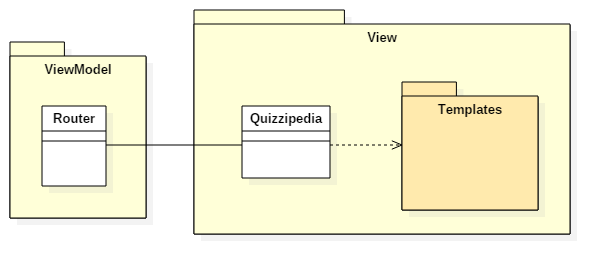
\includegraphics[scale=0.6]{../images/Quizzipedia.png}
		\end{center}
			\begin{itemize}
				\item\textbf{Funzione del componente:} pagina wrapper che visualizza gli elementi comuni a tutte le pagine e all'interno della quale vengono caricati dinamicamente gli altri templates tramite la componente Router.
				\item\textbf{Relazioni d'uso di altri componenti:} si relaziona con tutti gli altri templates e con la componente Router del ViewModel
			\end{itemize}	
	\newpage	
	
	\subsubsection{Package Templates}
		\begin{center}
			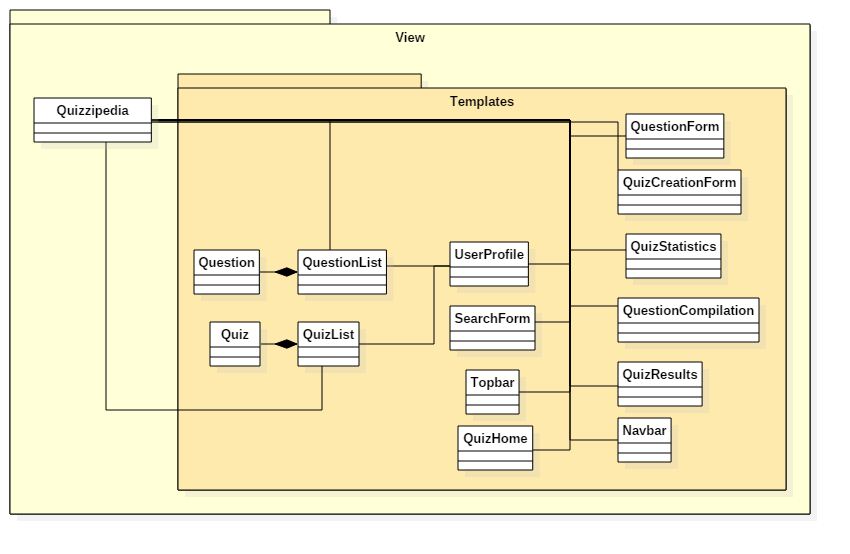
\includegraphics[scale=0.6]{../images/Templates.png}
		\end{center}
		\subsubsubsection{Classe QuestionList}
			\begin{itemize}
				\item\textbf{Funzione del componente:} visualizza una lista di domande
				\item\textbf{Relazioni d'uso di altri componenti:} composta da Question
			\end{itemize}
		\subsubsubsection{Classe Question}
			\begin{itemize}
				\item\textbf{Funzione del componente:} visualizza una domanda inserita in una lista
				\item\textbf{Relazioni d'uso di altri componenti:} usata solo da QuestionList per creare la lista
			\end{itemize}
		\subsubsubsection{Classe QuizList}
			\begin{itemize}
				\item\textbf{Funzione del componente:} visualizza una lista di quiz
				\item\textbf{Relazioni d'uso di altri componenti:} composta da Quiz
			\end{itemize}
		\subsubsubsection{Classe Quiz}
			\begin{itemize}
				\item\textbf{Funzione del componente:} visualizza un quiz inserito in una lista
				\item\textbf{Relazioni d'uso di altri componenti:} usata solo da QuizList per creare la lista
			\end{itemize}
		\subsubsubsection{Classe QuestionCompilation}
			\begin{itemize}
				\item\textbf{Funzione del componente:} visualizza una domanda e ne permette la compilazione
			\end{itemize}
		\subsubsubsection{Classe QuestionForm}
			\begin{itemize}
				\item\textbf{Funzione del componente:} visualizza il form per i dati di una domanda. Utilizzabile sia per la creazione che per la modifica della domanda (se viene modificata una domanda già esistente nei campi vengono inseriti i valori attuali)
			\end{itemize}
		\subsubsubsection{Classe QuizCreation}
			\begin{itemize}
				\item\textbf{Funzione del componente:} visualizza il form di creazione di un questionario
			\end{itemize}
		\subsubsubsection{Classe QuizResults}
			\begin{itemize}
				\item\textbf{Funzione del componente:} visualizza i risultati ottenuti in seguito alla compilazione di un quiz
			\end{itemize}
		\subsubsubsection{Classe LoginForm}
			\begin{itemize}
				\item\textbf{Funzione del componente:} visualizza un form per l'autenticazione, registrazione e recupero password di un utente
			\end{itemize}
		\subsubsubsection{Classe QuizResult}
			\begin{itemize}
				\item\textbf{Funzione del componente:} visualizza i risultati di un quiz appena compilato
			\end{itemize}		
		\subsubsubsection{Classe QuizHome}
			\begin{itemize}
				\item\textbf{Funzione del componente:} pagina di benvenuto di Quizzipedia
			\end{itemize}				
		\subsubsubsection{Classe QuizStatistics}
			\begin{itemize}
				\item\textbf{Funzione del componente:} permette la visualizzazione delle statistiche generali di un quiz
			\end{itemize}	
		\subsubsubsection{Classe SearchForm}
			\begin{itemize}
				\item\textbf{Funzione del componente:} visualizza una form per l’inserimento dei dati desiderati e l’avvio della ricerca
			\end{itemize}								
		\subsubsubsection{Classe Topbar}
			\begin{itemize}
				\item\textbf{Funzione del componente:} visualizza il menù orizzontale situato in cima all'applicazione
			\end{itemize}
		\subsubsubsection{Classe UserProfile}
			\begin{itemize}
				\item\textbf{Funzione del componente:} permette la visualizzazione del profilo utente e delle funzionalità ad esso associato
				\item\textbf{Relazioni d'uso di altri componenti:} fa uso dei templates QuizList e QuestionList 
			\end{itemize}			
					
			\newpage